\documentclass[a4paper,12pt]{book}

\usepackage[T1]{fontenc}	% Codifica di output
\usepackage[utf8]{inputenc}	% Codifica di input
\usepackage[italian]{babel}	% Lingua del documento

\usepackage{graphicx} % Grafica
\usepackage{xcolor} % \color

\usepackage{amsmath,amssymb,amsthm}	% Pacchetti per la matematica
\usepackage{units}

\usepackage{enumitem}

\usepackage{listings} % listati di codice
\lstdefinestyle{customc}{
	numbers=left,
	breaklines=true,
	frame=tb,
	xleftmargin=\parindent,
	language=C,
	showstringspaces=false,
	basicstyle=\footnotesize\ttfamily,
	keywordstyle=\bfseries\color{green!40!black},
	commentstyle=\itshape\color{purple!40!black},
	stringstyle=\color{orange}
}
\lstset{escapechar=@,style=customc}

\definecolor{light-gray}{gray}{0.95}

\begin{document}

\author{Bozzo Francesco \and Conti Samuele}
\title{Appunti di Programmazione 1\\Università degli Studi di Trento}
\date{Febbraio 2019}

\frontmatter
\maketitle
\tableofcontents

\mainmatter
\chapter{Introduzione all'informatica e al computer}
\section{Definizione di informatica}
\textit{Informàtica} s.f.[dal fr. informatique, comp. di informat(ion) e (automat)ique «informazione automatica»] è definita dalla Treccani come l’insieme dei vari aspetti scientifici e tecnici che sono specificamente applicati alla raccolta e al trattamento dell’informazione e in partica all’elaborazione automatica dei dati.

\section{Elementi di base}
Prima di addentrarsi nel mondo della programmazione è giusto comprendere (o per alcuni semplicemente ricordare) cos'è l'informatica e che cosa studia, nonchè quali sono i suoi obbiettivi ed i suoi concetti basilari: spesso capita di addentrarsi così tanto tra le righe di codice da perdere la limpidezza della visione generale su quello che si sta facendo.\\ 
A questo scopo abbiamo introdotto la definizione precedente e questo breve elenco dei concetti fondamentali di questa branca della scienza:
\begin{itemize}
	\item\textbf{Algoritmo}: un algoritmo è una sequenza precisa (=deterministica) e finita di operazioni, comprensibili da un esecutore, che portano alla realizzazione di un compito. L'esecutore non deve essere per forza di cose un computer, anche un libretto di istruzioni per montare un mobile è di per sè un algoritmo e l'umano che lo utilizza ne è l'esecutore.
	Le proprietà fondamentali di un algoritmo sono \textit{correttezza} ed \textit{efficienza}. Quando si opera con i calcolatori, gli algoritmi sono descritti utilizzando linguaggi che essi comprendono, i linguaggi di programmazione. 

	\item\textbf{Linguaggio di programmazione}: linguaggio specifico del campo informatico dedicato a descrivere le istruzioni ad un calcolatore, perciò deve essere deterministico e rigoroso; inoltre esso è caratterizzato da: 
	\begin{itemize}[noitemsep, nolistsep]
	    \item una \textit{sintassi}, cioè le regole che descrivono le stringhe di parole riconosciute dal linguaggio.
	    \item una \textit{semantica}, ovvero le regole per interpretazione delle stringhe e che descrivono i processi computazionali dell'esecutore.
	\end{itemize}
    I linguaggi di programmazione si possono definire di alto o basso livello a seconda della loro maggiore vicinanza al linguaggio naturale (alto livello, facilmente interpretabile dagli umani) o a quello della macchina (basso livello, facilmente interpretabile dai calcolatori).

	\item\textbf{Programma}: è un algoritmo codificato tramite uno specifico linguaggio. 
	Data la complessità di alcuni programmi, sono stati sviluppati linguaggi intermedi (di alto livello) più vicini al linguaggio naturale che facilitano la scrittura dei programmi e che poi possono essere tradotti in linguaggi di basso livello, ovvero più vicini alla macchina (ed interpretabili da essa); esempi sono lo pseudocodice ed i diagrammi di flusso.
\end{itemize}

\section{Il computer}
Ora che abbiamo chiarito velocemente i concetti fondamentali possiamo iniziare a parlare degli strumenti di cui la scienza dell'informatica fa uso. \\
Al giorno d'oggi esistono molti tipi di computer con caratteristiche e scopi diversi tra loro. Nonostante ciò, si possono distinguere alcune componenti comuni:
\begin{itemize}
	\item\textbf{CPU}: è l’unità di elaborazione del calcolatore (\textit{Central Processing Unit}), essa carica istruzioni da eseguire dalla memoria centrale, interpreta le istruzioni ed infine le esegue.
	Il lavoro della CPU è scandito da impulsi generati da un orologio interno (\textit{clock}): più è elevata la frequenza degli impulsi del \textit{clock} più sono le istruzioni eseguite nell’unità di tempo. Seppur da molti anni la velocità del \textit{clock} non si scosti di molto da $3\unit{GHz}$ per problemi relativi alla dissipazione del calore, tuttavia la velocità dei computer è andata comunque aumentando per via dell'introduzione di nuove architetture nella progettazione dei calcolatori (es.: computer \textit{multi-core}).
	\item\textbf{Memoria centrale (RAM)}: utilizzata per memorizzare dati e istruzioni, la \textit{Random Access Memory} è una memoria il cui tempo di accesso è indipendente dall’indirizzo del dato al quale si vuole accedere (al contrario delle memorie di massa). Si tratta di una memoria volatile, cioè il contenuto viene perso quando cessa l’alimentazione del sistema.
	\item\textbf{Bus di sistema}: interconnette tutti gli altri componenti, consentendo lo scambio di dati; esso è suddiviso in tre insiemi di \textit{linee}: 
	\begin{itemize}[noitemsep, nolistsep]
		\item Bus \textbf{dati}, per la trasmissione dei dati; 
		\item Bus \textbf{indirizzi}, un bus unidirezionale attraverso il quale la CPU decide in quale indirizzo scrivere o leggere i dati;
		\item Bus \textbf{di controllo}: trasporta informazioni relative alla modalità di trasferimento e alla temporizzazione.
	\end{itemize}
	In ogni istante è dedicato a collegare due unità, di cui una trasmette ed una riceve.
	\item\textbf{Periferiche di I/O}: ne esistono vari tipi: memorie di massa, monitor, tastiere, schede di rete, sensori etc.; non sono componenti fondamentali del calcolatore  ma permettono che esso venga utilizzato per un'enorme quantità di funzioni diverse.
	\item\textbf{Memorie ROM}: sono un tipo particolare di memorie su cui non è consentita la scrittura (\textit{Read Only Memory}). A esempio vengono utilizzate per memorizzare i firmware (software di basso livello, che comunicano direttamente con l'hardware, come il \textbf{BIOS}).
	
\end{itemize}

\section{La macchina di Von Neumann}
L'hardware sulla maggior parte dei computer moderni è progettato secondo lo schema della macchina di Von Neumann, facendo uso delle componenti indicate nell'elenco precedente. Il funzionamento di questa macchina si può riassumere schematicamente:
\begin{itemize} [noitemsep, nolistsep]
	\item le fasi di elaborazione si susseguono in modo sincrono rispetto all'orologio di sistema (\textit{clock}).
	\item durante ogni intervallo di tempo, l’unità di controllo (parte del processore) stabilisce la funzione da svolgere e l’intera macchina opera in maniera sequenziale (anche se le architetture più evolute prevedono esecuzione contempoarnea di più istruzioni).
	\item il Bus di sistema collega tutte le componenti del calcolatore tra loro ed alla CPU, la quale gestisce tutti i flussi in ingresso ed uscita. Usando una metafora musicale, essa è il direttore dell'orchestra.
\end{itemize}

\section{Astrazione e stratificazione}
I concetti di \textbf{astrazione} e \textbf{stratificazione} si sono rivelati fondamentali nell'evoluzione dell'informatica e nello sviluppo della tecnologia. Con il passare del tempo si sono costruiti calcolatori sempre più potenti, con la conseguente richiesta di software sempre più complessi, in grado di gestire appunto gli hardware più evoluti.\\
I programmatori hanno provveduto quindi ad una progressiva astrazione dei software stessi al fine di trovarsi ad operare su rappresentazioni semplificate della macchina. In aggiunta, anche i programmi stessi hanno iniziato a diventare sempre più onerosi da gestire.\\
La soluzione più comunemente adottata consiste nello stratificare in vari livelli di astrazione l'intero software. Un esempio lampante è l'architettuta dei moderni sistemi operativi, che si sviluppa partendo dalla macchina fisica fino al livello delle applicazioni utilizzate dall'utente finale.\\
Segue uno schema della tipica architettura a strati di un sistema operativo:
\begin{table}[!ht]
	\centering
	\label{Strati-OS}
	\begin{tabular}{c}
		\hline
		Programmi utente           \\ \hline
		Interprete dei comandi     \\ \hline
		File system                \\ \hline
		Gestione delle periferiche \\ \hline
		Gestione della memoria     \\ \hline
		Gestione dei processi      \\ \hline
		Macchina fisica            \\ \hline
	\end{tabular}
\caption{Architettura a strati di un sistema operativo}
\end{table}

\section{Rappresentazione dell'informazione}
L'ultimo argomento che tatteremo prima di passare al linguaggio C è la rappresentazione dell'informazione nella scienza informatica.\\
Essendo strutturalmente basato su dispositivi bistabili (con due stati stabili che possono essere utilizzati come base della rappresentazione), l'elaboratore elettronico può operare solo su sequenze di simboli binari. I due simboli convenzionalmente usati sono 0 e 1. Con il termine \textbf{BIT} (da \textit{Bynary digIT}) si intende l’unità elementare di informazione; istruzioni e dati sono rappresentati nel computer tramite sequenze di BIT. Un insieme di 8 bit si chiama \textbf{byte}. Sono spesso utilizzati i multipli del byte (secondo la notazione del sistema internazionale): \textit{KiloByte}($=1000$ byte), \textit{MegaByte}($=10^{6}$ byte), \textit{GigaByte}($=10^{9}$ byte).



\chapter{Introduzione alla programmazione C}
\chapter{Vettori e matrici}\label{vettori}
\section{Il concetto di array}
Il vettore, chiamato più comunemente \textbf{array}, è il più semplice esempio di dato strutturato, esso consiste in una sequenza di celle consecutive ed omogenee, ovvero una sorta di contenitore di tante variabili dello stesso tipo a cui è possibile accedere tramite il nome del vettore e l’indice della variabile racchiuso tra parentesi quadre.\\
Di per sé l'array nel linguaggio C non è effettivamente un tipo di dato, esso è un costruttore di tipo che permette di creare il tipo di dato appena descritto. \\
Un array si crea ponendo l'identificatore del tipo di elemnti che conterrà, il nome dell'array e la dimensione dello stesso tra parentesi quadre nel modo seguente:
\begin{lstlisting}[title={Implementazione di un array}]
//esempio con array con 3 interi
int vettore[3];

//esempio con array di 6 caratteri
char vettore_di_caratteri[6];

//esempio con array di 3 array di 2 interi
int vett[3][2];		//matrice 3*2
\end{lstlisting}
Si può usare come indice qualsiasi dato di tipo int e char.
Si possono creare array contenenti qualsiasi tipo di dato, sia esso \textit{built-in} o \textit{user-defined}, semplice o strutturato. Come si è appena visto nell'esempio, si possono creare anche array di array (detti comunemente array bidimensionali o matrici) e non c'è limite al numero di dimensioni che si possono sfruttare.

\section{Caratteristiche tecniche}
I singoli elementi di un array vengono trattati dal C come vere e proprie variabili (del tipo definito nella dichiarazione dell'array): essi dunque possono essere coinvolti in tutte le operazioni riguardanti il loro tipo. L'array invece non può essere coinvolto globalmente in operazioni nè di assegnamento nè di confronto. Il metodo più comune per agire sull'array intero spesso prevede l'utilizzo di cicli: in particolare il ciclo \textit{for} in cui il contatore viene utilizzato per scorrere l'array, come nell'esempio riportato qui sotto.
\begin{lstlisting}[title={Implementazione di un array}]
//si vuole inizializzare il seguente array di interi con una sequenza di 30
int voti[10];
int i;
for(i=0; i<10; i++){
    voti[i]=30;
}
\end{lstlisting}

\section{Stringhe}
Gli array vengono utilizzati anche per memorizzare stringe, i metodi di implementazione di qusto tipo di dato ed i suoi utilizzi saranno specificati in seguito.

\section{Punatori e array}
Esiste un legame stretto tra puntatori ed array: infatti, dichiarando un array \colorbox{light-gray}{a[n]}, è possibile accedere al suo \textit{i}-esimo elemento sia attraverso la scrittura \colorbox{light-gray}{a[i]} che \colorbox{light-gray}{*(a+i)}. Questo significa che l'identificatore \colorbox{light-gray}{a} in realtà è un puntatore \textit{read-only} alla prima cella dell'array. Si osservi il seguente esempio:
\begin{lstlisting}[title={Utilizzo di puntatori come array}]
int vett[5];
int *p;
// ottenimento indirizzo del vettore
p=&vett[0]; // analogo a p=vett;

// vett = &p; ERRORE: l'identificatore vett e' read-only

// accesso ad un elemento del vettore
*(p+2)=7;    // analogo a vett[2]=7

// chiamata a funzione
int result = funz_random(vett); // analogo a funz_random(&vett[0])

// definizione di funzione
funzione_2(int v[]); // analogo a funzione_2(int *v)
\end{lstlisting}

Nelle ultime due righe abbiamo visto per passare gli array alle funzioni si utilizza l'indirizzo del loro primo elemento.\\
Tuttavia va ricordato che puntatori e vettori hanno caratteristiche molto diverse: i primi sono un tipo di dato semplice, mentre i secondi sono un tipo di dato strutturato. Come si può osservare in seguito dunque non possono essere sottoposti alle stesse operazioni (in particolare assegnamento ed incremento):
\begin{lstlisting}[title={Differenze puntatori/array}]
int vett[5];
int *p;

// operazioni valide
p=vett;
p++;

// operazioni NON valide
// vett=p;
// vett++;
\end{lstlisting}

\section{Nota teorica}
Osservando da vicino la struttura dell'array, si nota che la principale limitazione consiste nel fatto che la dimensione di un array non può variare durante l'esecuzione del programma; questo implica che nel caso non si conoscano a tempo di compilazione le dimensioni di un input da memorizzare, si dovrà necessariamente sovrastimare le dimensioni dell'array per evitare il rischio di \textbf{overflow}, con conseguente spreco memoria.\\ 
Tale complicazione è dovuta alla complessità di realizzazione del compilatore di un linguaggio: se la macchina astratta (di un determinato linguaggio) conosce la quantità di memoria da allocare per un programma prima della sua esecuzione, 
potrà operare in maniera molto più efficiente, riservando a priori la memoria necessaria. In questo modo si evita la ricerca di  eventuali porzioni di memoria libera durante l'esecuzione del programma.\\
Questi concetti verranno ripresi e approfonditi nel capitolo \ref{memoriaDin}.
\chapter{Stringhe}

\section{Il concetto di stringa}
Come già visto nel capitolo \ref{vettori}, le stringhe sono strettamente legate al concetto di array, precisamente queste altro non sono che array di elementi di tipo char nella cui ultima cella è contenuto il carattere "$\backslash0$", identificato \textit{terminatore di stringa}.\\
Essendo usate comunemente, le stringhe hanno una serie di comandi che ne semplificano l'input e l'output (utilizzando il descrittore di formato \colorbox{light-gray}{\%s}).

\section{Operazioni con le stringhe}
Oltre a questo esiste una libreria standard interamente dedicata, \colorbox{light-gray}{string.h}, che comprende alcune utili funzioni quali \colorbox{light-gray}{strcpy()}, \colorbox{light-gray}{strlen()} e \colorbox{light-gray}{strcmp()}:
\begin{lstlisting}[title={Alcune operazione con le stringhe}]
char str1[5], str2[5];

fflush(stdin); // per Windows, da utilizzare prima di qualsiasi lettura di stringhe
scanf("%s", str1);
printf("%s", str1);

strcpy(str1, "cane"); //copia in str1 la stringa "cane"
strcpy(str2, str1); // copia il contenuto di str1 in str2

int lunghezza = strlen(str1); // restituisce la lunghezza di str1

bool uguali = strcmp(str1, "cane") == 0; // restituisce zero se uguali, >0 se str1>cane, <0 altrimenti
\end{lstlisting}
\section{Nota tecnica}
Considerando che l'ultimo carattere di una stringa deve essere il terminatore "$\backslash0$", e per scrivere una parola di \textit{n} lettere, bisogna utilizzare un array di lunghezza \textit{n+1}.

\chapter{Gestione file}
\section{Il concetto di file}
Il C gestisce le interazioni con le varie periferiche fisiche rappresentandole come \textbf{file} su cui agisce attraverso un meccanismo chiamato stream. Esso funziona come un'interfaccia consistente, cioè permette di interagire con tutti i tipi di periferiche allo stesso modo. Un file viene associato ad uno \textbf{stream} (flusso) tramite un'operazione di \textit{open}, (avvio delle comunicazioni tra software e periferica).\\
Il lingaggio C ha almeno 3 file costantemente aperti: \colorbox{light-gray}{stdin} (file di input), \colorbox{light-gray}{stdout} (file di output) e \colorbox{light-gray}{stderr} (file di registrazione degli errori).

\section{Come apriree chiudere un file}
Nella libreria standard del C esistono diversi strumenti per operare su file di testo e file binari. In entrambi i casi la funzione di apertura del flusso è però la medesima:
\begin{lstlisting}[title={Interfaccia funzione open()}]
FILE *file = fopen(<nome del file>, <tipo di apertura>);
\end{lstlisting}
La funzione \colorbox{light-gray}{fopen()} inoltre restituisce l'indirizzo della struttura file associata al flusso creato; se al contrario incontra qualche errore, restituisce \textit{NULL}.
Di seguito sono elencate le diverse modalità di apertura disponibili:
\begin{itemize}[noitemsep]
	\item \colorbox{light-gray}{"w"}: scrittura su file di testo.
	\item \colorbox{light-gray}{"r"}: lettura da file di testo.
	\item \colorbox{light-gray}{"a"}: aggiunta a file di testo.\footnote[1]{La modalità aggiunta è necessaria poichè ogni volta che un file viene aperto con comando "w" o "wb" il suo contenuto precedente viene eliminato}
	\item \colorbox{light-gray}{"wb"}: scrittura su file binari.
	\item \colorbox{light-gray}{"rb"}: lettura da file binari.
	\item \colorbox{light-gray}{"ab"}: aggiunta a file binari.
\end{itemize}
Esistono anche modalità avanzate (\colorbox{light-gray}{"w+"}, \colorbox{light-gray}{"r+"}, \colorbox{light-gray}{"a+"}) che permettono di modificare il cursore del file, decidendo in che posizione del file agire.\\
Ad ogni apertura di un file deve corrispondere una chiusura, attraverso la funzione \colorbox{light-gray}{fclose()}:
\begin{lstlisting}[title={Interfaccia funzione close()}]
fclose(<file>);
\end{lstlisting}
\section{Operazioni di lettura e scrittura su file}
Per la scrittura su un file di testo:
\begin{lstlisting}[title={Scrittura su file di testo}]
fputc(int c, file_output); // ritorna EOF come errore
fputs(stringa, file_output); // ritorna EOF come errore
fprintf(file_output, [formato_output], [var_list variabili]); // ritorna il numero di elementi scritti
\end{lstlisting}

Per la lettura da un file di testo:
\begin{lstlisting}[title={Lettura da file di testo}]
carattere = fgetc(file_input); // ritorna EOF come errore
fgets(stringa, lunghezza, file_input); // fino a newline o EOF; ritorna EOF come errore
fscanf(file_input, [formato_input], [var_list puntatori]); // ritorna il numero di elementi letti
\end{lstlisting}

Per verificare se ci si trova alla fine del file:
\begin{lstlisting}[title={Controllo fine file}]
int result = feof(file_input); // se la fine e' stata raggiunta, result assume un valore diverso da 0
\end{lstlisting}
Seppur la libreria standard del C offre questa funzione, quando bisogna leggere in insieme di elementi di cui non si conosce la dimensione è consigliato utilizzare \colorbox{light-gray}{fscanf()}. In particolare il controllo da eseguire è sul valore di ritorno di fscanf: se non sono stati letti tanti elementi quanti ci si aspetterebbe, allora il file è concluso.\\

Per lettura e scrittura su file binario:
\begin{lstlisting}[title={Controllo fine file}]
int n_read_elem = fread (void *ptr, len_elemento, n_elementi, file_input);
int n_written_elem = fwrite(void *ptr, len_elemento, n_elementi, file_input);
\end{lstlisting}
Una caratteristica interessante delle funzioni relative ai file binari è quella di offrire la possibilità di lettura/scrittura di tipi di dato, sia \textit{built-in} che \textit{user-defined}, con una singola istruzione.

\section{Alcuni esempi}
\begin{lstlisting}[title={Scrittura su file di testo}]
// creazione del puntatore alla struttura file
FILE *f_txt;
int x = 7;

// apertura file in modalita' scrittura con controllo sull'apertura
if ((f_txt=fopen("nomefile.txt", "w")) == NULL){
	printf("errore apertura file fase w");
}

// scrittura sul file
fprintf(f_txt, "numero_piccioni: %d", x);
fprintf(f_txt, "si puo' scrivere anche solo testo", NULL);

fclose(f_txt);
\end{lstlisting}

\begin{lstlisting}[title={Lettura da file di testo}]
FILE *f_txt;
if((f_txt=fopen("nomefile.txt", "r"))==NULL){
    printf("errore apertura file fase r");
}

int x;
char testo[20];
fscanf(f_txt, "%s: %d", &testo, &x); //lettura

fclose(f_txt);
\end{lstlisting}

\begin{lstlisting}[title={Append di un file di testo}]
FILE *f_txt;
if ((f_txt=fopen("nomefile.txt", "a")) == NULL){
    printf("errore apertura file fase a");
}

fprintf(f_txt, "testo aggiunto\n", NULL); // append

fclose(f_txt);
\end{lstlisting}

\begin{lstlisting}[title={File binari (.bin)}]
//creazione del puntatore alla struttura file
FILE *f_bin;
int x=12;

if ((f_txt=fopen("nomefile.bin", "wb")) == NULL){ 
    printf("errore apertura file fase wb");
}

// se si sta programmando su Windows, per poter controllare il file si deve comunque dichiararlo come .txt

fwrite(&x, sizeof(int), 1, f_bin); // scrittura sul file bin
fclose(f_bin);
\end{lstlisting}

\begin{lstlisting}[title={Scrittura di una struttura su file binario}]
typedef struct Tpunto {
    float x, y;
} Tpunto;

Tpunto p1;
p1.x = p2.x = 0.3;
FILE *f_bin;
if ((f_txt=fopen("nomefile.bin", "wb")) == NULL){ 
    printf("errore apertura file fase wb");
}

fwrite(&p1, sizeof(Tpunto), 1, f_bin); // scrittura binaria di un elemento Tpunto
fclose(f_bin);
\end{lstlisting}

\begin{lstlisting}[title={Lettura di una struttura da file binario}]
typedef struct Tpunto {
    float x, y;
} Tpunto;

Tpunto p1;
FILE *f_bin;
if((f_txt=fopen("nomefile.bin", "rb")) == NULL){
    printf("errore apertura file fase rb");
}

fread(&p1, sizeof(Tpunto), 1, f_bin); // lettura binaria di un elemento Tpunto

fclose(f_bin);
\end{lstlisting}

\begin{lstlisting}[title={Scrittura di una stuttura su file binario in append}]
typedef struct Tpunto {
    float x, y;
} Tpunto;

Tpunto p1;
p1.x = p2.x = 0.3;
FILE *f_bin;
if ((f_txt=fopen("nomefile.txt", "ab")) == NULL){
    printf("errore apertura file fase ab");
}

fwrite(&d2, sizeof(Tdato), 1, f_bin); // scrittura binaria di un elemento Tpunto

fclose(f_bin);
\end{lstlisting}
\chapter{Allocazione dinamica della memoria}\label{memoriaDin}
\section{Heap vs stack}
Il linguaggio C permette al programmatore di utilizzare dei meccanismi di allocazione e deallocazione dinamica della memoria per gestire situazioni in cui un’allocazione statica sarebbe svantaggiosa. Un semplice esempio riguarda quei casi in cui non si è a conoscenza, al tempo della compilazione, delle dimensioni con cui si svilupperanno certe strutture dati durante l'esecuzione.\\
A differenza delle \textbf{variabili automatiche} che vengono memorizzate nello \textit{stack}, le variabili allocate dinamicamente si trovano nell'\textbf{heap}.\\
Naturalmente da grandi poteri derivano grandi responsabilità: ogni istruzione di allocazione deve essere accompagnata da una successiva istruzione di deallocazione. Nel caso contrario si possono riscontrare errori molto subdoli e nascosti come la produzione di \textit{garbage} (ovvero celle di memoria piene ma non recuperabili) e di \textit{dangling references} (ovvero celle di memoria a cui si può accedere da più puntatori, con il rischio di modificarle non intenzionalmente).

\section{Allocazione e deallocazione...}
Nel caso di fallimento di un'operazione di allocazione viene restituito il valore \textit{NULL}.\\
\`{E} possibile utilizzare le istruzioni di deallocazione ad un puntatore se e solo se esso contiene un indirizzo sull'heap assegnato dinamicamente.
\subsection{... in C}
Nel linguaggio C è necessario includere la libreria \textit{stdlib.h} per utilizzare le istruzioni per allocazione e deallocazione:
\begin{lstlisting}[title={Allocazione e deallocazione dinamica di una variabile in C}]
tipo* ptr_var = (tipo*) malloc(sizeof(tipo));
free(ptr_var);
\end{lstlisting}
\begin{lstlisting}[title={Allocazione e deallocazione dinamica di un vettore in C}]
tipo* ptr_arr = (tipo*) malloc(sizeof(tipo)*len_array);
free(ptr_arr);
\end{lstlisting}
Nota: \colorbox{light-gray}{sizeof} è un operatore unario che restituisce il numero di byte che occupa in memoria il tipo di dato che gli viene fornito.

\subsection{... in C++}
Nel linguaggio C++ le istruzioni per allocazione e deallocazione sono:
\begin{lstlisting}[title={Allocazione e deallocazione dinamica di una variabile in C++}]
tipo* ptr_var = new tipo;
delete ptr_var;
\end{lstlisting}
\begin{lstlisting}[title={Allocazione e deallocazione dinamica di un vettore in C++}]
tipo* ptr_arr = new tipo[];
delete [] ptr_arr;
\end{lstlisting}

\section{Tre sezioni di memoria}
Per ricapitolare, esistono principalmente tre sezioni di memoria in un programma C/C++:
\begin{itemize}
	\item \textit{Memoria automatica}: contiene le variabili che vengono allocate/deallocate automaticamente nello stack quando viene invocata/termina la funzione in cui sono definite.
	\item \textit{Memoria dinamica}: viene allocata a run-time nello heap dagli operatori presentati precedentemente.
	\item \textit{Memoria statica}: contiene le variabili statiche e globali.
\end{itemize}



\chapter{Teoria sulla complessità}
\section{La funzione tempo di esecuzione}
Dato un qualsiasi algoritmo, è possibile ottenere la funzione $T(n)$ ad esso associata, ossia la \textbf{funzione tempo di esecuzione} rispetto alla dimensione dell'input $n$. Questa funzione prende in considerazione solamente il numero di istruzioni e non aspetti dinamici d'esecuzione.\\
Studiando l'andamento asintotico di $T(n)$, si può notare che rilevante ciò che cresce più velocemente:
\textit{es} $T(n)=a+bn+cn^2 \Rightarrow T(n) = \varTheta(n^2)$.
\subsection*{Il caso peggiore, migliore e medio}
Si possono costruire \textit{tre} funzioni $T(n)$:
\begin{itemize}[noitemsep, nolistsep]
	\item $T_\text{peggiore}(n)$ nel caso peggiore
	\item $T_\text{migliore}(n)$ nel caso migliore
	\item $T_\text{medio}(n)$ nel caso medio
\end{itemize}
\vspace{10px}
Di ciascuna di esse si può determinare l'andamento asintotico attraverso le notazioni successivamente fornite.

\section{Notazione per l'andamento asintotico}
\subsection*{Notazione limite superiore $O$-grande}
\begin{gather*}
f(n)=O(g(n))\\
\text{se } \exists n_0 >0, \exists c_2 >0 \text{ tc. } f(n)\leq c_2 g(n) \forall n>n_0
\end{gather*}

\subsection*{Notazione limite inferiore $\varOmega$-omega}
\begin{gather*}
f(n)=\varOmega(g(n))\\
\text{se } \exists n_0 >0, \exists c_1 >0 \text{ tc. } f(n)\geq c_1 g(n) \forall n>n_0
\end{gather*}

\subsection*{Notazione limite superiore e inferiore $\varTheta$-theta}
\begin{gather*}
f(n)=\varTheta(g(n))\\
\text{se } \exists n_0 >0, \exists c_1>0,c_2>0 \text{ tc. } c_1g(n)\leq f(n)\leq c_2 g(n) \forall n>n_0
\end{gather*}

\section{Definizione di complessità}

\paragraph{Complessità di un algoritmo} La complessità di un algoritmo equivale alla misura del numero di istruzioni da eseguire per risolvere il problema.

\paragraph{Complessità di un problema} La complessità di un problema equivale alla complessità del migliore algoritmo che lo risolve.

\section{Le equazioni di ricorrenza}
Quando si deve analizzare un algoritmo ricorsivo del tipo \textit{divide et impera}, non è possibile scrivere l'espressione analitica di $T(n)$. Bisogna utilizzare un'equazione di ricorrenza:
\begin{equation*}
T(n) = 
\begin{cases}
\varTheta(1), n\le c\\
aT\Bigl(\frac{n}{b}\Bigr)+D(n)+C(n), n>c
\end{cases}
\end{equation*}
Dove:
\begin{itemize}[noitemsep, nolistsep]
	\item $c$ costante
	\item $a$ numero di problemi generati da \textit{divide}
	\item $b$ dimensione dei sottoproblemi rispetto a quello originale
	\item $D(n)$ tempo impiegato per dividere il sottoproblema (operazione di \textit{divide})
	\item $C(n)$ tempo impiegato per ricombinare le soluzioni dei sottoproblemi (operazione di \textit{combina})
\end{itemize}

\section{Risoluzione delle equazioni di ricorrenza}

\subsection{Metodo iterativo}
Questo metodo consiste nel calcolare $T(n)$ in funzione delle sue iterazioni successive.
\paragraph{Esempio}

\begin{flalign*}
&\begin{cases}
T(1) = 1\\
T(n) = 1 + T(\frac{n}{2})
\end{cases}\\
&\hspace{30px}T\Bigl(\frac{n}{2}\Bigr) = T\Bigl(\frac{n}{4}\Bigr)+1
\quad T\Bigl(\frac{n}{4}\Bigr) = T\Bigl(\frac{n}{8}\Bigr)+1 \hspace{\linewidth}\\
&\hspace{30px}T(n) = T\Bigl(\frac{n}{4}\Bigr)+1+1\\
&\hspace{30px}T(n) = T\Bigl(\frac{n}{8}\Bigr)+1+1+1
\end{flalign*}
Dunque, alla \textit{i}-esima iterazione: $T(n)=T\bigl(\frac{n}{2^i}\bigr)+i$\\
Per ottenere il limite asintotico superiore, ci si ferma quando: $\frac{n}{2^i}=1 \Rightarrow n=2^i \Rightarrow i=\log_2n$\\
\begin{equation*}
T(n) = T(1)+\log_2n= 1+\log_2n \Rightarrow T(n)=O(\log_2n)
\end{equation*}

\subsection{Metodo dell'esperto}
Si definisce il seguente teorema:
\begin{gather*}
a,b\in\mathbb{N}, a\ge1, b\ge2, c\in\mathbb{R}, \beta\in\mathbb{R}, c\ge0, \beta\ge0\\
T(n)=
\begin{cases}
aT\bigl(\frac{n}{b}\bigr)+cn^\beta, n>1\\
d, n\le1
\end{cases}
\end{gather*}
Posto $\alpha = \log_ba = \frac{\log a}{\log b}$, si ha che:
\begin{equation*}
T(n) = 
\begin{cases}
\varTheta(n^\alpha), \alpha>\beta\\
\varTheta(n^\alpha\log_2n), \alpha=\beta\\
\varTheta(n^\beta), \alpha<\beta
\end{cases}
\end{equation*}

\subsection{Metodo dell'albero di ricorsione}

\paragraph{Esempio}
\begin{flalign*}
T(n) = 
&\begin{cases}
\varTheta(1), n\le c\\
3T(\frac{n}{4})+\varTheta(n^2), n>c
\end{cases}
\end{flalign*}

\begin{center}
	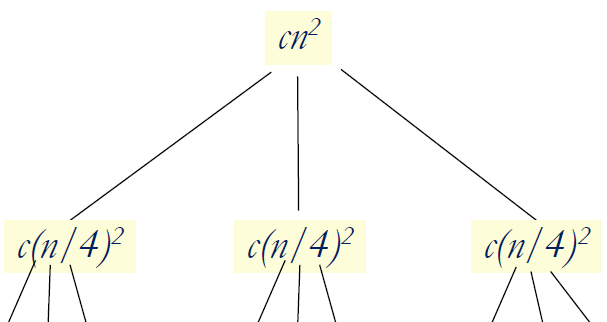
\includegraphics[width=0.5\textwidth]{img/albero_di_ricorsione.png}
\end{center}

\begin{enumerate}[noitemsep]
	\item si calcola il numero dei nodi per livello: $3^i$ in questo caso.
	\item si calcola il peso di ciascun livello moltiplicando ill numero di nodi per livello per il peso di ciascun nodo di quel livello
	\item si calcola il numero di livelli: $log_4n+1$ in questo caso. Si noti che il $4$ è il valore di $b$ dell'equazione di ricorrenza. Il numero dei livelli deve essere dimostrato per induzione.
	\item si calcola il numero di foglie: in questo caso $3^\text{altezza}$, dove l'altezza dell'albero è il numero di livelli meno 1.
	\item T(n) è pari dunque alla somma dei pesi di $i-1$ livelli più la somma dei pesi delle foglie.
\end{enumerate}

\subsection{Metodo della sostituzione}
Per applicare il metodo di sostituzione:
\begin{enumerate}
	\item si indovini la soluzione $\varTheta(f(n))$ (si consiglia il metodo dell'esperto).
	\item dimostrare per induzione la validità del limite superiore, inferiore o entrambi in base alla richiesta.
\end{enumerate}

\paragraph{Esempio}
\begin{flalign*}
&\begin{cases}
T(1) = 1\\
T(n) = n + 2T(\frac{n}{2})
\end{cases}
\end{flalign*}
Si ha: $T(n) = \varTheta(n\log_2n) \Rightarrow c_1n\log_2n\le T(n) \le c_2n\log_2n $ per il teorema dell'esperto.\\
Si studia il limite superiore trovando per quali $c>0$ vale $T(n) \le c_2n\log_2n$:
\begin{enumerate}[noitemsep, nolistsep]
	\item Si prova il caso base.
	\item Si utilizza l'ipotesi induttiva: $k<n, T(k)\le ck\log_2k$.
\end{enumerate}
Quindi: $T(n)=2T(\frac{n}{2})+n \le 2c\frac{n}{2}\log_2\frac{n}{2}+n$, e così via.\\
Per il limite inferiore il procedimento è del tutto analogo:
\begin{enumerate}[noitemsep, nolistsep]
	\item Si prova il caso base.
	\item Si utilizza l'ipotesi induttiva: $k<n, T(k)\ge dk\log_2k$.
\end{enumerate}
\chapter{Algoritmi di ricerca e ordinamento}

\section{Algoritmi di ricerca}
Un \textbf{algoritmo di ricerca} permette di trovare un elemento avente determinate caratteristiche all'interno di un insieme di elementi identificati da una chiave.

\subsection{Ricerca sequenziale}
Consiste nel scorrere tutti gli elementi fino a quando non si trova quello desiderato:
\begin{lstlisting}[title={Ricerca sequenziale}]
int sequential_search(char v[], int len, char key){
    int i;
    for (i=0; i<len; i++){
        if (v[i] == key){
            return i;
        }
    }
    return -1;
}
\end{lstlisting}
In questo caso, la funzione $T(n)$ è pari:
\begin{itemize}[noitemsep, nolistsep]
	\item nel caso peggiore: $n$.
	\item nel caso migliore $1$.
	\item nel caso medio $\frac{n}{2}$.
\end{itemize}

\subsection{Ricerca sequenziale con sentinella}
Come sopra, ma evita un confronto: posiziono al termine del vettore l'elemento da cercare:
\begin{lstlisting}[title={Ricerca sequenziale con sentinella}]
// la funzione chiamante deve assicurare la presenza di un elemento vuoto alla fine del vettore
int sequential_search_sentinella(char v[], int len, char key){
    int i;
    v[len] = key;
    for (i=0; v[i]!=key; i++){	}

    if (i == len) {
        return -1;
    }
    return i;
}
\end{lstlisting}

\subsection{Ricerca sequenziale su vettore ordinato}
Questa ricerca sfrutta il fatto di ricevere un vettore ordinato in input:
\begin{lstlisting}[title={Ricerca sequenziale su vettore ordinato}]
int sequential_search_order(char v[], int len, char key){
    int i;
    for (i=0; key>=v[i] && i<len; i++){
        if (v[i] == key){
            return i;
        }
    }
    return -1;
}
\end{lstlisting}

\subsection{Ricerca binaria}
Si presuppone che l'input sia un insieme ordinato di elementi con la possibilità di accesso casuale (\textit{es.} array):
\begin{lstlisting}[title={Ricerca binaria}]
int binary_search(char v[], int len, char key){
    int bottom = 0;
    int top = len - 1;
    int mid;

    while (bottom <= top){
        mid = (top + bottom) / 2;
        if (v[mid] == key) {
            return mid;
        }
        if (key < v[mid]){
            top = mid - 1;
        } else {
            bottom = mid + 1;
        }
    }
    return -1;
}
\end{lstlisting}
In questo caso, la funzione $T(n)$ è pari:
\begin{itemize}[noitemsep, nolistsep]
	\item nel caso peggiore: $\log_2n$.
	\item nel caso migliore $1$.
	\item nel caso medio $\log_2n$.
\end{itemize}

\section{Algoritmi di ordinamento}

\subsection{Insertion sort}
L'algoritmo di \textbf{insertion sort} permette di riordinare in maniera efficiente un piccolo insieme di elementi.
La complessità asintotica dell'algoritmo:
\begin{itemize}[noitemsep, nolistsep]
	\item caso medio: $\varTheta(n^2)$
	\item caso peggiore: $\varTheta(n^2)$
\end{itemize}
Dato un vettore $v$, l'algoritmo si basa sul costruisce (a partire dall'indice zero di $v$) un sottoarray ordinato.
\begin{lstlisting}[title={Insertion sort}]
void insertion_sort(char v[], int len){
    int i, j;
    char temp;
    for (i=1; i<len; i++){
        j = i-1;
        temp = v[i];
        while (j>=0 && v[j]>temp){
            v[j+1] = v[j];
            j--;
        }
        v[j+1] = temp;
    }
}
\end{lstlisting}

\subsection{Merge Sort}
Viene qui di seguito presentata la versione ricorsiva dell'algoritmo di ordinamento \textbf{merge sort}. Esso è definito come un algoritmo \textit{divide et impera}, in quanto:
\begin{itemize}[noitemsep]
	\item[divide]: separa la sequenza di $n$ elementi in 2 da $\frac{n}{2}$.
	\item[impera]: ordina le due sottosequenze generate da divide.
	\item[combina]: unisce le due sottosequenze rispettivamente ordinate in un tempo $\varTheta(n)$.
\end{itemize}
Utilizzando l'implementazione ricorsiva, sono indispensabili i casi base:
\begin{itemize}[noitemsep, nolistsep]
	\item dato un vettore da un elemento, esso è gia ordinato.
	\item dato un vettore di due elementi, o è già ordinato o è necessario invertirne gli elementi.
\end{itemize}
La complessità asintotica dell'algoritmo:
\begin{itemize}[noitemsep, nolistsep]
	\item caso medio: $\varTheta(n\log n)$
	\item caso peggiore: $\varTheta(n\log n)$
\end{itemize}
\begin{lstlisting}[title={Merge Sort}]
// passo di combina, con allocazione dinamica della memoria
void merge(char v[], int p, int mid, int r){
    int i, j, k;
    int len1 = mid-p+1;
    int len2 = r-mid;
    char *L = new char[len1+1];
    char *R = new char[len2+1];

    for (i=0; i<len1; i++){
        L[i] = v[p+i];
    }
    for (i=0; i<len2; i++){
        R[i] = v[mid+1+i];
    }
    L[len1] = R[len2] = (char)'z'; // sentinella

    i = j = 0;
    for (k=p; k<=r; k++){
        if (L[i] < R[j]){
            v[k] = L[i++];
        } else {
            v[k] = R[j++];
        }
    }
    delete [] L;
    delete [] R;
}

void merge_sort(char v[], int p, int r){
    // caso base: 1 elemento
    if (r-p <= 0){
        return;
    // caso base: 2 elementi
    } else if (r-p == 1) {
        if (v[p] > v[r]){
            char temp = v[p];
            v[p] = v[r];
            v[r] = temp;
        }
        return;
    // caso induttivo
    } else {
        int mid = (p+r)/2;
        merge_sort(v, p, mid);
        merge_sort(v, mid+1, r);
        merge(v, p, mid, r);
    }
}

\end{lstlisting}

\subsection{Teorema della complessità nel caso pessimo di un algoritmo di ordinamento}
La complessità nel caso pessimo di un algoritmo di ordinamento sul posto che confronta e scambia elementi consecutivi è $\varOmega(n^2)$. Algoritmi più efficienti richiedono scambi di elementi lontani fra loro.
\chapter{Liste}
\section{Implementazione della struttura}
Una \textbf{lista} è una struttura di dati astratta che permette di contenere un insieme di elementi. Attraverso la gestione dinamica della memoria non è inoltre necessario specificare la dimensione della struttura al momento della compilazione (attraverso costanti o \textit{define}). A differenza di un array, in cui i propri elementi occupano celle contigue di memoria, gli elementi di una lista possono essere localizzati posizioni diverse dell'heap.\\
Una lista può essere implementata in due diverse modalità:
\begin{itemize}
	\item \textbf{semplicemente concatenata (sc)}: ogni elemento ha un puntatore all'elemento successivo
	\item \textbf{doppiamente concatenata (dc)}: ogni elemento ha due puntatori: uno all'elemento precedente e l'altro all'elemento successivo
\end{itemize}

Seppur la presenza di un ulteriore puntatore nell'implementazione \textit{dc} possa sembrare un'inutile ridondanza, in realtà permette di semplificare e ottimizzare alcuni algoritmi.\\
Entrambe le strutture presentano un metodo di accesso \textit{sequenziale} e non casuale (tipico degli array).

\begin{lstlisting}[title={Implementazione lista singolarmente concatenata}]
typedef struct Tnodo{
    Tdato dato;
    Tnodo *next;

    // costruttori
    Tnodo(Tdato d);
    Tnodo(Tdato d, Tnodo *n);
} Tnodo;
typedef Tnodo *ListaSemplicementeConcatenata;
\end{lstlisting}

\begin{lstlisting}[title={Implementazione lista doppiamente concatenata}]
struct Tnodo {
    Tdato dato;
    Tnodo *next;
    Tnodo *prev;
    
    // costruttori
    Tnodo(Tdato);
    Tnodo(Tdato d, Tnodo *p, Tnodo *n);
};
typedef Tnodo *ListaDoppiamenteConcatenata;
\end{lstlisting}

\section{Ricerca di un elemento}
Come anticipato precedentemente, si può accedere ad un elemento di una lista in maniera sequenziale e non casuale. Dunque, nel caso peggiore, la complessità dell'algoritmo è $O(n)$.
\begin{lstlisting}[title={Ricerca di un elemento di una lista semplicemente/doppiamente concatenata}]
Lista ricerca(const Lista ls, Tdato d){
    Lista temp = ls;
    while (!is_empty_lista(temp)){
        if (temp->dato.isEqual(d)) {
            return temp;
        }
        temp = temp->next;
    }
    return NULL;
}
\end{lstlisting}


	
\section{Inserimento di un elemento}
Nel caso di una lista \textit{sc}, quando la si scorre per inserire un elemento in coda o in ordine, è necessario tenere memoria anche dell'elemento precedente a quello in cui si sta visitando.\\
\`{E} molto oneroso effuare operazioni in coda: è necessario infatti visitare tutta la lista.
\begin{lstlisting} [title={Inserimento in testa, in coda, ordinato in una lista \textit{sc}}]
Lista inserisci_in_testa(Lista ls, Tdato d){
    return new Tnodo(d, ls);
}

Lista inserisci_in_coda(Lista ls, Tdato d){
    Lista temp = ls;
    if (is_empty_lista(temp)){
        return inserisci_testa(ls, d);
    }
    while (temp->next != NULL){
        temp = temp->next;
    }
    temp->next = new Tnodo(d, NULL);
    return ls;
}

Lista inserisci_ordinato(Lista ls, Tdato d){
    Lista temp = ls;
    Lista pred = NULL;
    if (is_empty_lista(temp)){
        return inserisci_testa(ls, d);
    }
    while ((!is_empty_lista(temp)) && temp->dato.isLowerThan(d)){ 
        //isLowerThan=metodo per verificare se dato e' minore di d
        pred = temp;
        temp = temp->next;
    }
    if (is_empty_lista(temp)){
        pred->next = new Tnodo(d, NULL);
    } else if (temp==ls) {
        return inserisci_testa(ls, d);
    } else {
        pred->next = new Tnodo(d, temp);
    }
    return ls;
}
\end{lstlisting}
\vspace{20px}
Invece, nel caso di una lista doppiamente concatenata, è possibile risalire all'elemento precedente attraverso al campo \textit{prev}:
\begin{lstlisting}[title={Inserimento in testa, in coda, ordinato in una lista \textit{dc}}]
ListaDoppia inserisci_testa_doppia(ListaDoppia ls,Tdato d){
    ListaDoppia temp = new Tnodo(d, NULL, ls);
    if (ls != NULL){
        ls->prev = temp;
    }
    return temp;
}

ListaDoppia inserisci_coda_doppia(ListaDoppia ls, Tdato d){
    if (ls == NULL){
        return inserisci_testa_doppia(ls, d);
    }
    ListaDoppia temp = ls;
    while (temp->next != NULL){
        temp = temp->next;
    }
    temp->next = new Tnodo(d, temp, NULL);
    return ls;
}

ListaDoppia inserisci_ord_doppia(ListaDoppia ls, Tdato d){
    if (ls == NULL){
        return inserisci_testa_doppia(ls, d);
    }
    ListaDoppia temp = ls;
    ListaDoppia old = NULL;
    while ((temp!=NULL) && (temp->dato.isLowerThan(d))){
        old = temp;
        temp = temp->next;
    }
    Tnodo *t = NULL;
    if (temp == NULL){
        t = new Tnodo(d, old, NULL);
        old->next = t;
    } else {
        if (temp->prev != NULL){
            t = new Tnodo(d, temp->prev, temp);
            temp->prev->next = t;
            temp->prev = t;
        } else {
            t = new Tnodo(d, NULL, temp);
            temp->prev = t;
            return t;
        }	
    }	
    return ls;
}
\end{lstlisting}

\section{Rimozione di un elemento}
Come per l'inserimento, è molto oneroso effuare operazioni in coda: è necessario infatti visitare tutta la lista.
\begin{lstlisting}[title={Eliminazione di un elemento, di un elemento in testa e in coda con lista \textit{sc}}]
Lista delete_el(Lista ls, Tdato d){
    Lista temp = ls;
    Lista pred = NULL;
    while (!is_empty_lista(temp)){
    if (temp->dato.isEqual(d)){
        if (pred != NULL){
            pred->next = temp->next;
            delete temp;
            return ls;
        } else {
            Lista res = temp->next;
            delete temp;
            return res;
        }
    }
    pred = temp;
    temp = temp->next;
    }
}

Lista delete_testa(Lista ls){
    if (ls != NULL) {
        Lista temp = ls;
        ls = ls->next;
        delete temp;
    }
    return ls;
}

Lista delete_coda(Lista ls){
    if (ls != NULL) {
        Lista temp = ls;
        Lista pred = NULL;
        while (!is_empty_lista(temp->next)){
            pred = temp;
            temp = temp->next;
        }
        if (pred == NULL){
            return delete_testa(ls);
        }
        delete temp;
        pred->next = NULL;
    }
    return ls;
}
\end{lstlisting}

\begin{lstlisting}[title={Eliminazione di un elemento, di un elemento in testa e in coda con lista \textit{dc}}]
ListaDoppia delete_el_doppia(ListaDoppia ls, Tdato d){
    if (ls != NULL){
        if (ls->dato.isEqual(d)){
            return delete_testa_doppia(ls);
        }
        ListaDoppia temp = ls;
        while ((temp!=NULL) && (!temp->dato.isEqual(d))){
            temp = temp->next;
        }
        if (temp != NULL){
            if (temp->next != NULL){
                temp->next->prev = temp->prev;
            }
            temp->prev->next = temp->next;
            delete temp;
        }
    }
    return ls;
}

ListaDoppia delete_testa_doppia(ListaDoppia ls){
    ListaDoppia temp = ls->next;
    delete ls;
    temp->prev = NULL;
    return temp;
}

ListaDoppia delete_coda_doppia(ListaDoppia ls){
    if (ls != NULL){
        ListaDoppia temp = ls;
        while (temp->next != NULL){
            temp = temp->next;
        }
        if(temp->prev != NULL){
            temp->prev->next = NULL;
            delete temp;
        } else {
            delete temp;
            return init_doppia();
        }
    }
    return ls;
}
\end{lstlisting}

\section{Calcolare la lunghezza di una lista}
Sia per le liste \textit{sc} e \textit{dc} l'implementazione è la medesima:
\begin{lstlisting}
unsigned int length_lista(const Lista ls){
    unsigned int len = 0;
    Lista temp = ls;
    while (!is_empty_lista(temp)){
        len++;
        temp = temp->next;
    }
    return len;
}
\end{lstlisting}

\chapter{Liste circolari}
Il concetto di \textbf{lista circolare} è del tutto analogo a quello di una lista semplicemente o doppiamente concatenata: l'unica differenza è data dal fatto che l'ultimo elemento della lista è legato al primo. Dunque, bisogna porre attenzione a come scorrere la lista per evitare di incorrere in loop infiniti.

\section{Implementazione della struttura}
Principalmente si possono distinguere due implementazioni per la lista circolare:
\begin{itemize}[noitemsep, nolistsep]
	\item attraverso liste semplicemente o doppiamente concatenate.
	\item attraverso un vettore.
\end{itemize}
\begin{lstlisting}[title={Implementazione di una lista circolare in C++}]
typedef struct ListaCircolare{
    // campi
    Tdato v[MAX];
    unsigned int n;     // numero di elementi nella lista
    unsigned int testa; // indice dell'elemento in testa
    unsigned int coda;  // indice dell'elemento successivo alla coda

    // costruttore
    ListaCircolare(){
        n = testa = coda = 0;
    }
    
    // metodi
    ...
} ListaCircolare;
\end{lstlisting}

\section{Ricerca di un elemento}
\begin{lstlisting}[title={Metodo per la ricerca di un elemento in una lista circolare}]
bool contains(Tdato d){
    int j;
    for (j=0; j<n; j++){
        if (v[(testa+j) % MAX] == d){
            return true;
        }
    }
    return false;
}
\end{lstlisting}

\section{Inserimento di un elemento}
\begin{lstlisting}[title={Metodo per l'inserimento in testa in una lista circolare}]
void insertFirst(Tdato d){
    if (!isFull()){
        testa = (testa-1) % MAX;
        if (testa < 0){
            testa += MAX;
        }
        v[testa] = d;
        n++;
    }
}
\end{lstlisting}
\begin{lstlisting}[title={Metodo per l'inserimento in coda in una lista circolare}]
void insertLast(Tdato d){
    if (!isFull()){
        v[coda] = d;
        coda = (coda+1) % MAX;
        n++;
    }
}
\end{lstlisting}

\section{Rimozione di un elemento}
\begin{lstlisting}[title={Metodo per la rimozione della testa da una lista circolare}]
void removeFirst(){
    if (!isEmpty()){
        testa = (testa+1) % MAX;
        n--;
    }
}
\end{lstlisting}
\begin{lstlisting}[title={Metodo per la rimozione della coda da una lista circolare}]
void removeLast(){
    if (!isEmpty()){
        coda = (coda-1) % MAX;
        if (coda < 0){
            coda += MAX;
        }
        n--;
    }
}
\end{lstlisting}

\section{Calcolare la lunghezza della lista}
Si può notare com'è immediato restituire la lunghezza di una lista circolare:
\begin{lstlisting}[title={Metodo per restituire la lunghezza di una lista circolare}]
int length(){
    return n;
}
\end{lstlisting}

\section{Controllo lista piena/vuota}
In modo analogo, anche qui il campo $n$ (contenente il numero di elementi) torna utile:
\begin{lstlisting}[title={Metodo per controllare se la lista circolare è vuota}]
bool isEmpty(){
    return n == 0;
}
\end{lstlisting}
\begin{lstlisting}[title={Metodo per controllare se la lista circolare è piena}]
bool isFull(){
    return n == MAX;
}
\end{lstlisting}

\chapter{Stack e code}

\section{Stack}
\subsection{Definzione e implementazione}
Lo \textbf{stack} (in italiano \textbf{pila}) è una struttura dati astratta di tipo \textbf{LIFO} (\textit{Last In First Out}).\\
Sia per definizione, che per problemi di ottimizzazione, lo stack prevede un solo punto di accesso per l'inserimento e la rimozione di un elemento: la testa.\\
La pila può essere implementata con:
\begin{itemize}[noitemsep, nolistsep]
	\item \textit{array}: gestione statica della memoria; limite massimo di dimensione.
	\item \textit{liste}: gestione dinamica della memoria; occupazione variabile e non limitata.
\end{itemize}

\subsection{Funzioni}
Le principali funzioni che uno stack deve fornire sono:
\begin{itemize}[noitemsep]
	\item \textit{init()}: inizializza la struttura.
	\item \textit{push()}: inserisce in elemento in testa con complessità $O(1)$.
	\item \textit{pop()}: elimina un elemento dalla testa con complessità $O(1)$.
	\item \textit{top()}: restituisce l'elemento in testa.
	\item \textit{isEmpty()}: verifica se lo stack è vuoto.
	\item \textit{isFull()}: verifica se lo stack è pieno.
	\item \textit{remove()}: rimozione di un elemento (utilizzando un secondo stack).
\end{itemize}

\subsection{Applicazioni}
Alcuni utilizzi dello stack riguardano:
\begin{itemize}[noitemsep]
	\item trasformazione da espressioni in notazione infissa a postfissa.
	\item valutazione di espressioni in notazione postfissa.
	\item implementazione iterativa di algoritmi riguardo gli alberi binari di ricerca.
	\item struttura degli ambienti di chiamata delle funzioni in runtime.
\end{itemize}

\section{Code}
\subsection{Definizione}
La \textbf{coda} (in inglese \textbf{queue}) è una struttura dati astratta di tipo \textbf{FIFO} (\textit{First In First Out}).\\
Sia per definizione, che per ottimizzare sia l'estrazione che l'inserimento, la queue prevede 2 punti di accesso:
\begin{itemize}[noitemsep, nolistsep]
	\item \textit{front} (in italiano \textit{testa}) per l'estrazione.
	\item \textit{rear} (in italiano \textit{coda}) per l'inserimento.
\end{itemize}

\subsection{Implementazione}
La coda può essere implementata attraverso:
\begin{itemize}[noitemsep]
	\item liste concatenate.
	\item liste circolari.
\end{itemize}
\begin{lstlisting}[title={Implementazione di una coda attraverso liste concatenate}]
typedef struct Queue {
    Tnodo *head;
    Tnodo *tail;
} Queue;
\end{lstlisting}

\subsection{Funzioni}
Le principali funzioni che una queue deve fornire sono:
\begin{itemize}[noitemsep]
	\item \textit{enqueue()}: inserisce un elemento nel rear con complessità $O(1)$.
	\item \textit{dequeue()}: estrae un elemento dal front con complessità $O(1)$.
	\item \textit{queueIsEmpty()}: verifica se la coda è vuota.
	\item \textit{queueIsFull()}: verifica se la coda è piena (se implementata con liste circolari).
	\item \textit{front()}: restituisce l'elemento in front.
\end{itemize}
\chapter{Alberi binari di ricerca}

\section{Definizioni di albero}
\begin{itemize}[noitemsep]
	\item Un \textit{albero} è un grafo non orientato, connesso e privo di cicli.
	\item Attraverso la \textit{ricorsione}:
	\begin{itemize}[noitemsep, nolistsep]
		\item l'insieme vuoto $\phi$ è un albero binario.
		\item $T_s$ e $T_d$ sono alberi binari ed $r$ è un nodo: la terna $(r, T_s, T_d)$ è un albero binario.
	\end{itemize}
	\item Un \textit{albero binario di ricerca} è un albero in cui ogni nodo ha al più due figli tale che ogni nodo è maggiore (o uguale) dei valori dei nodi del suo sottoalbero sinistro e minore (o uguale) dei valori dei nodi del suo sottoalbero destro.
\end{itemize}
Alcune sigle per identificare un albero binario di ricerca sono \textit{ABR} e \textit{BST} (dall'inglese \textit{binary search tree}).

\begin{lstlisting}[title={Implementazione di un albero binario di ricerca}]
typedef struct Tnodo {
Tdato dato;
Tnodo *sx;
Tnodo *dx;
Tnodo *parent; //non utilizzato in lab
} Tnodo;
typedef ABR *Tnodo;
\end{lstlisting}

\section{Proprietà}
\begin{enumerate}[noitemsep]
	\item Un ABR non ha una rappresentazione univoca. Alcuni rappresentazioni infatti risultano più bilanciate di altre.
	\item Un ABR si dice \textit{bilanciato} se i suoi nodi sono equamente distribuiti, senza eccedere in altezza.
	\item \textit{Altezza}: lunghezza massima tra radice e una foglia, ossia $h = n_\text{livelli}-1$.
	\item \textit{Foglia}: nodo senza figli.
	\item \textit{Radice}: nodo senza padre.
	\item \textit{Cammino} di un ABR: somma per ciascun nodo la sua distanza dalla radice.
	\item Il percorso dalla radice ad ogni foglia è unico.
\end{enumerate}


\section{Algoritmi}
\subsection{Visita in preordine}
\begin{lstlisting}[title={Visita in preordine di un ABR}]
void visita_preordine(BST tree){
    if (tree != NULL){
        tree->dato.print();
        visita_preordine(tree->sx);
        visita_preordine(tree->dx);
    }
}
\end{lstlisting}

\subsection{Visita in ordine}
Attraverso una stampa della visita in ordine si ottiene un elenco ordinato.
\begin{lstlisting}[title={Visita in ordine di un ABR}]
void visita_ordine(BST tree){
    if (tree != NULL){
        visita_ordine(tree->sx);
        tree->dato.print();
        visita_ordine(tree->dx);
    }
}
\end{lstlisting}

\subsection{Visita in postordine}
\begin{lstlisting}[title={Visita in postordine di un ABR}]
void visita_postordine(BST tree){
    if (tree != NULL){
        visita_postordine(tree->sx);
        visita_postordine(tree->dx);
        tree->dato.print();
    }
}
\end{lstlisting}

\subsection{Visita in level-ordine}
Nella visita in level-ordine si percorrono i nodi per ciascun livello.

\subsection{Ricerca di un elemento}
In maniera ricorsiva, cerca fra i sottoalberi di un nodo. Nel caso peggiore ha complessità $O(h)$.
\begin{lstlisting}[title={Ricerca ricorsiva di un elemento in un ABR}]
Tnodo *search_element(BST tree, Tdato d){
    if (tree->dato.isEqual(d)){
        return tree;
    } else if (d.isLowerThan(tree->dato)){
        return search_element(tree->sx, d);
    } else {
        return search_element(tree->dx, d);
    }
}
\end{lstlisting}

\subsection{Ricerca del minimo}
Si continua iterativamente a percorrere il sottoalbero sinistro. Nel caso peggiore ha complessità $O(h)$.
\begin{lstlisting}[title={Ricerca del minimo in un ABR}]
Tdato minimo(BST tree){
    BST temp = tree;
    while (temp->sx != NULL){
        temp = temp->sx;
    }
    return temp->dato;
}
\end{lstlisting}

\subsection{Ricerca del massimo}
Si continua iterativamente a percorrere il sottoalbero destro. Nel caso peggiore ha complessità $O(h)$.
\begin{lstlisting}[title={Ricerca del massimo in un ABR}]
Tdato massimo(BST tree){
    BST temp = tree;
    while (temp->dx != NULL){
        temp = temp->dx;
    }
    return temp->dato;
}
\end{lstlisting}

\subsection{Ricerca del successore e predecessore}
Per implementare i seguenti algoritmi, nell'implementazione dell'ABR si necessita del riferimento ai genitori. Nel caso peggiore ha complessità $O(h)$.

\subsection{Calcolo dell'altezza}
L'algoritmo consiste nel percorrere tutti i percorsi, cercandone il più lungo.
\begin{lstlisting}[title={Calcolo dell'altezza in un ABR}]
int altezza(BST tree){
    if (tree == NULL){
       return -1; // dovuto alla definizione di altezza
    } else {
       return max(1+altezza(tree->sx),1+altezza(tree->dx));
    }
}
\end{lstlisting}

\subsection{Inserimento di un elemento}
Nel caso peggiore ha una complessità $O(h)$.
\begin{lstlisting}[title={Inserimento di un elemento in un ABR}]
BST insert_node(BST tree, Tdato d){
    if (tree == NULL){
        return new Tnodo(d, NULL, NULL);
    } else {
        tree = insert_ric(tree, d);
        return tree;
    }
}

// la funzione deve restituire un BST, in quanto non basta creare un nuovo nodo: bisogna anche collegarlo al precedente
BST insert_ric(BST tree, Tdato d){
    if (tree == NULL){
        return new Tnodo(d, NULL, NULL);
    } else {
        if (d.isGreaterThan(tree->dato)){
            tree->dx = insert_ric(tree->dx, d);
        } else {
            tree->sx = insert_ric(tree->sx, d);
        }
    }
    return tree;
}
\end{lstlisting}

\subsection{Conta numero di nodi}
\begin{lstlisting}[title={Conta numero di nodi di un ABR}]
int conta_nodi(BST tree){
    if (tree == NULL){
        return 0;
    } else {
        return 1 + conta_nodi(tree->sx) + conta_nodi(tree->dx);
    }
}
\end{lstlisting}

\subsection{Cancellazione di un elemento}
Di seguito si descrive l'algoritmo per la \textit{cancellazione} di un elemento $z$:
\begin{itemize}
	\item caso 1: se $z$ non ha figlio $\textit{sx}$:
	\begin{enumerate}
		\item se $\text{dx != NULL}$, sostituisci $\textit{dx}$ a $z$.
		\item se ha entrambi i figli $\textit{NULL}$, nessun problema
	\end{enumerate}
	\item caso 2: se $z$ ha solo figlio $\textit{sx}$, sostituisci $\textit{sx}$ a $z$.
	\item caso 3: se $z$ ha due figli. Sia $y$ il successore di $z$ ($y$ ha necessariamente sottoalbero sinistro nullo e si trova nel sottalbero destro di $z$):
	\begin{enumerate}
		\item se $y$ è il diretto figlio destro di $z$: sostituisci $y$ (mantenendo il suo sottoalbero destro) a $z$.
		\item se $y$ non è il diretto figlio destro di $z$: scambia $y$ con il diretto figlio destro di $z$; sostituisci $y$ (mantenendo il suo sottoalbero destro) a $z$.
	\end{enumerate}	
\end{itemize}


\chapter{Hashing}
La \textbf{tabella di hash} è una struttura che permette di effettuare ricerca e inserimento $O(1)$ sotto \textit{ipotesi ragionevoli}: non si basa su confronti e mantenimento dell'ordine dei dati. Se mal costruita, la ricerca nel caso peggiore è $\varTheta(n)$.\\
La ricerca consiste nell'associare ad ogni \textit{chiave} i suoi rispettivi \textit{dati satellite}. Un semplice esempio è un database finalizzato a memorizzare dei dispositivi: ciascun record infatti ha associato una chiave (es. MAC Address) e dei dati satellite (es. marca, caratteristiche, ecc.). L'insieme di chiavi $U$ deve essere piccolo.

\section{Tavole a indirizzamento diretto}
Il metodo attraverso una \textbf{tavola a indirizzamento diretto} utilizza un vettore $V$ di puntatori, di dimensione $|U|$.\\
Quando si inserisce un elemento nella tavola, viene generato dinamicamente il corrispondente putatore ai dati satellite, che viene inserito nella cella di $V$ corrispondente alla propria chiave. Dunque vi è una corrispondenza biunivoca tra celle di $V$ e le chiavi possibili.

\paragraph{Vantaggi}
\begin{itemize}
	\item le operazioni di inserimento, ricerca e cancellazione risultano di costo unitario.
\end{itemize}
\paragraph{Svantaggi}
\begin{itemize}
	\item il costo oneroso iniziale nel settare a \textit{NULL} tutti gli elementi di $V$.
	\item se la cardinalità di $U$ è troppo elevata, non si può utilizzare la tavola ad indirizzamento diretto in quanto occuperebbe troppa memoria.
\end{itemize}

\section{Tabella di Hash}
Con la \textbf{tabella di hash} si introduce la \textbf{funzione di hashing} $F$: riceve in input una chiave $c$ e restituisce l'indice del vettore $V$ che punta ai dati satellite di $c$. A differenza della tavola a indirizzamento diretto, la chiave non viene più utilizzata come indice di $V$.

\paragraph{Collisioni}
Seppur il numero di chiavi utilizzate sia piccolo rispetto a $|U|$, $F$ può presentare delle collisioni. Si incontra una \textit{collisione} quando a chiavi diverse vengono assegnati gli stessi dati satellite. Minore è la probabilità di trovare collisioni, maggiore è qualità di $F$.

\paragraph{Chaining}
La tecnica di \textit{chaining} permette di risolvere il problema delle collisioni. Ad ogni elemento dell'immagine di $F$ viene associata una lista concatenata $L$ di chiavi (con i corrispondenti dati satellite): nel caso della ricerca, prima si applica $F$ e poi, attraverso un algoritmo $\varTheta(n)$, si cerca l'elemento con la chiave voluta all'interno della lista associata.\\
Il \textit{fattore di carico} $alpha = \frac{n}{m}$, dove $n$ rappresenta il numero di chiavi e $m$ rappresenta il numero di celle della tavola, è pari alla lunghezza media di una lista $L$. Nel caso peggiore, la ricerca nella lista $\varTheta(1+\alpha)$. Dunque, più ridotte solo le liste, più veloce è la ricerca. La soluzione ottimale è trovare una funzione $F$ che distribuisce le chiavi in maniera più uniforme possibile.\\
Un esempio riguarda la seguente funzione di hash: $h(k) = k \% m + 1$. Se $m$ si trova vicino ad una potenza di 2, allora $h(k)$ non ha una distribuzione uniforme delle proprie chiavi.

\paragraph{Funzione di hash universale}
Ogni funzione di hash ha delle distribuizioni di probabilità non uniformi per alcuni input. Si utilizza perciò la \textit{funzione di hash universale} se per ogni coppia di chiavi distinte vi sono al più $\frac{|H|}{m}$ funzioni di hash che causano collisione fra le due chiavi. $H$ è l'insieme delle funzioni di hash utilizzate, da cui se ne sceglie una casualmente.

\appendix
\chapter{Tabella di precedenza degli operatori}

\begin{center}
	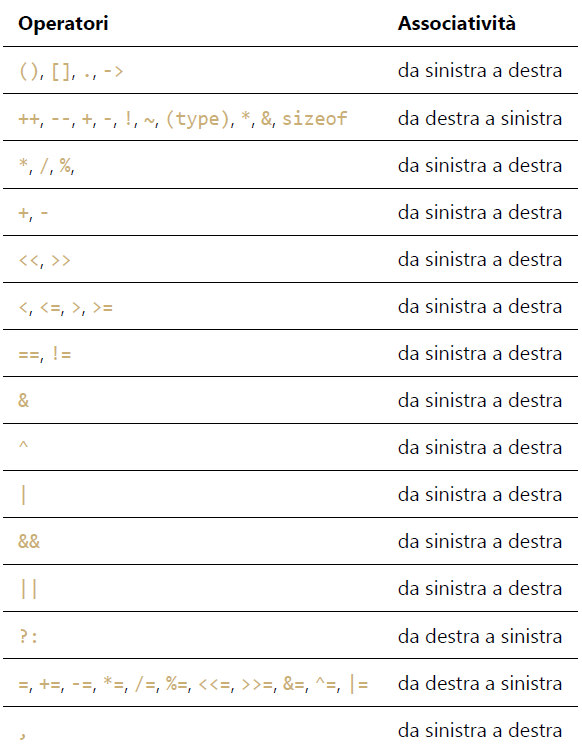
\includegraphics[width=0.8\textwidth]{img/operatori.png}
\end{center}

\backmatter
% bibliography, glossary and index would go here.

\end{document}